% Contributors: Jie Li, Yadin Rozov
% Contributors: Kevin Wu, Emily Jin
% Contributors: Jenny Chen, Collin Burns, Nav Ravindranath
% Contributors: Eric Bolton, Xinyuan Cao
% Contributors: Carolina Zheng
\section{Hardness of \emph{k}-means}

In this section, we show that the $k$-means problem is NP-hard. To do
so, we first demonstrate that NAE-3SAT* $\le_p$ Generalized 2-means, and
then that the Generalized 2-means instance constructed in the reduction
of NAE-3SAT* can be solved by 2-means. Since NAE-3SAT* is a decision
problem which is known to be NP-hard, this establishes the NP-hardness
of $k$-means.

To motivate the definition of the Generalized $k$-means problem, we
first reformulate the original $k$-means problem. We initially defined
the $k$-means problem as follows.

\begin{mdframed}
    \underline{\textbf{$k$-means (Formulation 1)}}
    
    \vspace{0.5em} \underline{Input}:
    $\{x_1, \ldots, x_n\} = S \subset \bbR^d$, positive integer $k$
    
    \vspace{0.5em} \underline{Output}: $T \subset \bbR^d$, $|T| = k$
    
    \vspace{0.5em} \underline{Goal}: minimize $\text{cost}(T) :=
    \sum\limits_{s \in S} \min\limits_{t \in T} \norm{s - t}^2$
\end{mdframed}

Equivalently, rather than only outputting a set $T$ of cluster centers,
we could instead output a partition of the input set $S$. This gives a
second formulation of $k$-means.

\begin{mdframed}
    \underline{\textbf{$k$-means (Formulation 2)}}
    
    \vspace{0.5em} \underline{Input}:
    $\{x_1,\ldots,x_n\} = S \subset \bbR^d$, positive integer $k$
    
    \vspace{0.5em} \underline{Output}: $P_1, \ldots, P_k \subset [n],
    ~\bigcup_{j=1}^k P_j = [n],
    ~P_j \cap P_{j'} = \emptyset ~\text{for}~ j \ne j';$

    $\quad \mu_1, \ldots, \mu_k \in \bbR^d,
    ~\mu_j ~\text{is the center of the points in cluster}~ P_j$
    
    \vspace{0.5em} \underline{Goal}: minimize
    $\text{cost}(P_1, \ldots, P_k, \mu_1, \ldots, \mu_k) :=
    \sum\limits_{j=1}^k \sum\limits_{i \in P_j} \norm{x_i - \mu_j}^2$
\end{mdframed}

Finally, we make use of the following fact to remove the necessity to
explicitly know the cluster centers.

\begin{fact}
    $\E \norm{X - \E X}^2 = \frac{1}{2} \E_{X,Y} \norm{X - Y}^2
    \quad (X, Y ~\text{i.i.d.})$
\end{fact}

\begin{proof}
    \begin{align*}
        \E_{X,Y} \norm{X - Y}^2
        &= \E_{X,Y} \left[(X - Y)^2\right] \\
        &= \E_X \E_Y \left[X^2 + Y^2 - 2 X Y\right] \\
        &= \E X^2 + \E Y^2 - 2 \E_X \E_Y [X Y] \\
        &= 2 \left[\E X^2 - (\E X)^2\right] \\
        &= 2 \E \left[(X - \E X)^2\right] \\
        &= 2 \E \norm{X - \E X}^2
    \end{align*}
\end{proof}

Observing that each cluster center $\mu_j := \frac{1}{|P_j|}
\sum_{i \in P_j} x_i$ can be thought of as an expectation of the points
in belonging to $P_j$, and applying the previous fact, we see that
\begin{align*}
    \sum_{j=1}^{k} \sum_{i \in P_j} \norm{x_i - \mu_j}^2
    &= \sum_{j=1}^{k} \sum_{i \in P_j} \norm{x_i - \frac{1}{|P_j|}
        \sum_{i' \in P_j} x_{i'}}^2 \\
    &= \sum_{j=1}^{k} \frac{1}{2 |P_j|} \sum_{i,i' \in P_j}
        \norm{x_i - x_{i'}}^2
\end{align*}
which leads to yet another formulation of $k$-means.

\begin{mdframed}
    \underline{\textbf{$k$-means (Formulation 3)}}
    
    \vspace{0.5em} \underline{Input}:
    $\{x_1,\ldots,x_n\} = S \subset \bbR^d$, positive integer $k$
    
    \vspace{0.5em} \underline{Output}: $P_1, \ldots, P_k \subset [n],
    ~\bigcup_{j=1}^k P_j = [n],
    ~P_j \cap P_{j'} = \emptyset ~\text{for}~ j \ne j'$
    
    \vspace{0.5em} \underline{Goal}: minimize
    $\text{cost}(P_1, \ldots, P_k) := \sum\limits_{j=1}^{k}
    \frac{1}{2 |P_j|} \sum\limits_{i,i' \in P_j} \norm{x_i - x_{i'}}^2$
\end{mdframed}

A slight modification of this last formulation leads to the Generalized
$k$-means problem; instead of using the squared distance penalty term
$\norm{x_i - x_{i'}}^2$, we can specify the penalties as an $n \times n$
matrix $D$ with the entry $D_{ii'}$ giving the penalty for points $x_i$
and $x_{i'}$.

\begin{mdframed}
    \underline{\textbf{Generalized $k$-means}}
    
    \vspace{0.5em} \underline{Input}:
    $n \times n$ symmetric matrix $D$, positive integer $k$
    
    \vspace{0.5em} \underline{Output}: $P_1, \ldots, P_k \subset [n],
    ~\bigcup_{j=1}^k P_j = [n],
    ~P_j \cap P_{j'} = \emptyset ~\text{for}~ j \ne j'$
    
    \vspace{0.5em} \underline{Goal}: minimize
    $\text{cost}(P_1, \ldots, P_k) := \sum\limits_{j=1}^{k}
    \frac{1}{2 |P_j|} \sum\limits_{i,i' \in P_j} D_{ii'}$
\end{mdframed}

\subsection{Review of NP-hard problems}
\begin{enumerate}
\item Problems that are NP-hard admit polynomial time
  reductions from all other problems in NP.
\item To carry out such a necessary reduction that proves a problem is NP-hard, the following steps can used (\cite{cor2009}): 
\begin{enumerate}
\item Given an instance $\alpha$ of a problem $A$ that has previously
  been proven to be NP-hard ($A \in NP$), use a polynomial time algorithm to transform it to an instance $\beta$ of problem $B$ .
\item Run a decision algorithm for $B$ on instance $\beta$ 
\item Use the answer for $\beta$ to get $\alpha$
\end{enumerate} 
\end{enumerate} 

For a more complete review of complexity and hardness please go to
reference \cite{cor2009} chapter 34.

Our goal is to show that the 2-means problem is NP hard:

\begin{theorem}\label{2-means-np-hard}
2-means clustering is an NP-hard optimization problem
\end{theorem} 

Approach to the problem is based on \cite{das2008}.  To prove this we
will start with the known NP-hard problem of 3SAT and show a reduction
from it to the NAE-3SAT* problem.  From that problem we will show a
reduction to the Generalized 2-means problem and finally show a
reduction from that to the 2-means problem. \\

In each reduction  we need to show how an instance of the known NP-hard problem can be modified in polynomial time into an instance of the problem we want
to show is NP-hard, and vice versa. In other words, we must show that the reduction maps a 'yes'
instance of the known problem to a 'yes' instance of the new problem
and 'no' instance of the known problem to a 'no' instance of the new
problem. Note since the set NP is a set of \emph{decision problems}, the
input of an instance of a problem must include the decision threshold
for the problem.

We'll briefly review NP-completeness, only to the extent necessary to
set the stage for this proof.  A more thorough treatment can found in
a computational complexity course. As a consequence of the Cook-Levin
Theorem, which pointed to the first NP-hard problem, we know that SAT
and variations, such as 3SAT and NAE 3-SAT, are NP-hard.

\subsection{Hardness proof preliminaries}
\begin{definition}[3SAT]
\item \underline{Input}:  A 3-CNF Boolean formula over $n$ literals. 
\begin{itemize}
\item 3-CNF (3-Conjunctive Normal Form): A Boolean formula that can be expressed as an \emph{AND} over
  $m$ clauses, each of which is an \emph{OR} over exactly 3 literals.
\end{itemize}
\item \underline{Output}: \emph{True} if there exists, \emph{False} if not.
\end{definition}

\begin{definition}[NAE 3-SAT] \emph{NAE 3-SAT} or
  \emph{not-all-equal-3SAT} is a 3SAT formula, with the additional
  requirement that, in each clause at least one literal is true and at
  least one literal is false.  This removes the case where all three
  literals in a clause are true.   
\end{definition}

\begin{definition}[NAE 3-SAT*] 
A boolean formula $\phi$ containing $n$ literals $x_1,...x_n$.
Exactly 3 literals for each of $m$ clauses.  Each pair of variables
$x_i$, $x_j$ appears in at most 2 clauses.  Once as $(x_i,x_j)$ or
$(\neg x_i, \neg x_j)$ and once as  $(x_i,\neg x_j)$ or $(\neg x_i,
x_j)$. 
\end{definition}

\begin{definition}[Generalized 2-means]
\item \underline{Input}: $n \times n$ matrix, ``distance matrix'' with
    elements $D_{ii'} =$ distance between object $i$ and object $i'$
\item \underline{Output}: Partition of objects into $P_1$ and $P_2$
\item \underline{Goal}: minimize $cost(P_1,P_2) := \sum\limits_{j=1}^{2}
    \frac{1}{2|P_j|} \sum\limits_{i,i' \in P_j} D_{ii'}$. 
\end{definition}


\begin{lemma}[Hardness of NAE-3SAT*] \label{np-nae-3-sat}
See \cite{das2008}. (??)
\end{lemma}

\subsection{Hardness of generalized 2-means}

For any instance $\phi$ of $x_1,...x_n$ of NAE-3SAT* we construct a
$2n \times 2n$ distance matrix $D_{\alpha,\beta}$ as below where
$\alpha,\beta \in x_1,...x_n, \neg x_1,....,\neg x_n$.  Note that
because the definition of NAE-3SAT* requires that each pair of
variables $x_i$, $x_j$ appears in at most 2 clauses, once as
$(x_i,x_j)$ or $(\neg x_i, \neg x_j)$ and once as  $(x_i,\neg x_j)$ or
$(\neg x_i, x_j)$ , the matrix is uniquely defined for a given
$\phi$. 
\begin{definition}[Distance matrix for generalized
    2-means] \label{2-means-distance-matrix} Define
  $D(\phi)$ by:
\begin{align}
  D_{\alpha,\beta} = \begin{cases}
    0 & \textrm{if } \alpha = \beta\\
    1+\Delta  & \mbox{if } \alpha = \overline{\beta} \\
    1+\delta  & \mbox{if } \alpha \sim \beta \\
    1 & \textrm{otherwise}.
  \end{cases}
\end{align}
Where $ \alpha \sim \beta$ means that either $\alpha$ and $\beta$
occur together in a clause or $\alpha$ and $\overline{\beta} $ occur
together in a clause, where:
\begin{align}
  \Delta = \frac{5m}{5m + 2n} \quad\textrm{and}
  \quad\delta = \frac{1}{5m  + 2n}.
\end{align}
\end{definition}
Note that above implies that $0 < \delta < \Delta < 1$ and also:
\begin{align}
4 \delta m < \Delta \le 1 - 2 \delta n.
\end{align}

Consider the following example matrix generated from the clause $x_1 \vee \bar{x_2} \vee x_3$, where the diagonal is filled with 0s (where $\alpha=\beta$).

\begin{table}[H]
\begin{tabular}{lllllll}
                       & $x_1$                      & $x_2 $                     & $x_3 $                    & $\bar{x_1}$                      & $\bar{x_2}$                      & $\bar{x_3}$                     \\ \cline{2-7} 
\multicolumn{1}{l|}{$x_1$} & \multicolumn{1}{l|}{0} & \multicolumn{1}{l|}{1}  & \multicolumn{1}{l|}{1+$\delta$}  & \multicolumn{1}{l|}{1+$\Delta$}  & \multicolumn{1}{l|}{$1+\delta$}  & \multicolumn{1}{l|}{1}  \\ \cline{2-7} 
\multicolumn{1}{l|}{$x_2$} & \multicolumn{1}{l|}{1}  & \multicolumn{1}{l|}{0} & \multicolumn{1}{l|}{1}  & \multicolumn{1}{l|}{1+$\delta$}  & \multicolumn{1}{l|}{1+$\Delta$}  & \multicolumn{1}{l|}{1+$\delta$}  \\ \cline{2-7} 
\multicolumn{1}{l|}{$x_3$} & \multicolumn{1}{l|}{1+$\delta$}  & \multicolumn{1}{l|}{1}  & \multicolumn{1}{l|}{0} & \multicolumn{1}{l|}{1}  & \multicolumn{1}{l|}{1+$\delta$}  & \multicolumn{1}{l|}{1+$\Delta$}  \\ \cline{2-7} 
\multicolumn{1}{l|}{$\bar{x_1}$} & \multicolumn{1}{l|}{1+$\Delta$}  & \multicolumn{1}{l|}{1+$\delta$}  & \multicolumn{1}{l|}{1}  & \multicolumn{1}{l|}{0} & \multicolumn{1}{l|}{1}  & \multicolumn{1}{l|}{1+$\delta$}  \\ \cline{2-7} 
\multicolumn{1}{l|}{$\bar{x_2}$} & \multicolumn{1}{l|}{1+$\delta$}  & \multicolumn{1}{l|}{1+$\Delta$}  & \multicolumn{1}{l|}{1+$\delta$}  & \multicolumn{1}{l|}{1}  & \multicolumn{1}{l|}{0} & \multicolumn{1}{l|}{1}  \\ \cline{2-7} 
\multicolumn{1}{l|}{$\bar{x_3}$} & \multicolumn{1}{l|}{1}  & \multicolumn{1}{l|}{1+$\delta$}  & \multicolumn{1}{l|}{1+$\Delta$}  & \multicolumn{1}{l|}{1+$\delta$}  & \multicolumn{1}{l|}{1}  & \multicolumn{1}{l|}{0} \\ \cline{2-7} 

\end{tabular}

\end {table}

We want to reformulate Generalized k-means from a minimization problem to a decision problem to prove satisfiability, so we prove the following lemma.
\begin{lemma} \label{generalized-2-means-cost}
$\phi$ is NAE-3SAT* satisfiable if and only if $D(\phi)$ admits a
generalized 2-means cost of $cost(\phi) = n - 1 + \frac{2\delta
  m}{n}$. 
\end{lemma}

\begin{proof}
Partition the corresponding matrix object ($2n$ object) for the
NAE-3SAT* satisfied $\phi$ into two partitions; one for all the
literals that are assigned \textit{true} and a second for all literals
that are assigned \textit{false}.  Since each literal is represented
twice we have $|P_1| = |P_2| = n$.   By definition of the NAE-3SAT*,
each clause contributes one pair to $P_1$ and pair to $P_2$.   Also
this leads to the fact that the distances between pairs can only be 1,
$1+\delta$, with $m$ instances of the later and the fact that the two
clusters have identical costs. So we get that 
\begin{align*}
cost(P_1,P_2) &= \sum_{j=1}^{2} \frac{1}{2|P_j|} \sum_{i,i' \in P_j}
D_{ii'}\\ 
&= \frac{1}{2n}( 2 {n \choose 2} + 2m\delta ) + \frac{1}{2n}( 2 {n
  \choose 2} + 2m\delta ) \\ 
&= \frac{ n (n-1) } {n} + \frac{2 m \delta}{n} \\
&= n - 1 +  \frac{2 m \delta}{n}
\end{align*}
\end{proof}

\begin{lemma} \label{different-partitions}
For any partition $P_1$ and $P_2$, WLOG $P_1$ contains a variable and
its negation, with $cost(P_1,P_2) \ge n - 1 + \frac{\Delta}{2n} > n -
1 + \frac{2m\delta}{n} = cost(\phi).$ 
\end{lemma}

\begin{proof}
Let $n' = |P_1|$.  Note
\begin{align*}
cost(P_1,P_2) &\ge \frac{1}{n'}({n' \choose 2} + \Delta ) +
\frac{1}{2n-n'}{2n-n' \choose 2}  \\ 
&= n - 1 + \frac{\Delta}{n'} \ge n-1 +\frac{\Delta}{2n}.
\end{align*}
\end{proof}

\begin{figure}
    \centering
    \includegraphics[width=10cm]{chapter_1/files/KmeansNAE3SAT.png}
\centering
    \caption{Partition of True and False literals, with blue lines meaning a cost of $1+\delta$, demonstrating that each clause contributes only $1+\delta$ cost within its cluster.}
    \label{fig:my_label}
\end{figure}


\begin{lemma} \label{satisfiable-instance}
If $D(\phi)$  admits a generalized 2-means cost of $cost(\phi) \le n -
1 + \frac{2\delta m}{n}$, then $\phi$ is a satisfiable instance of
NAE-3SAT*. 
\end{lemma}

\begin{proof}
Let $P_1$ and $P_2$ be the partition with cost $\le n - 1 +
\frac{2\delta m}{n}$.  First note that $P_1$ and $P_2$ do not contain
a variable and its negation and $|P_1| = |P_2| = n$.  The cost of
clustering $P_1$ and $P_2$ is:
\begin{align*}
  \frac{2}{n} \left[ {n \choose 2} + \delta \sum_{\textrm{clauses}} 
  \begin{cases}
    1 & \textrm{if clause is split across $P_1$ and $P_2$}\\  
    3 & \textrm{otherwise} \\ 
  \end{cases}\right]
\end{align*}
Since $cost(P_1, P_2) \le n - 1 + \frac{2\delta m}{n}$, it follows that all
clauses are split between $P_1$ and $P_2$.  That is, every clause has
at least one literal in $P_1$ and one literal in $P_2$.  Therefore,
the assignment that sets all of the $P_1$ to true and all of $P_2$ to
false is a valid NAE-3SAT* assignment. 
\end{proof}



\subsection{Generalized 2-means to 2-means}
We will use the hardness of generalized 2-means to show the hardness
of 2-means by embedding $D(\phi)$.
\begin{fact}
Note that any $n \times n$ symmetric matrix $D$ can be embedded in
$l_2^2$ iff $u^TDu  \le 0$ for all $u \in \mathbb{R}^n$ s.t. $\sum u_i
= 0$. 
\end{fact}
\begin{proof}[Proof as homework exercise]
\end{proof}

\begin{fact} \label{d-phi-fact}
For $D(\phi)$, the following holds:
\begin{align*}
u^TDu &= \sum_{\alpha, \beta} u_\alpha u_\beta D_{\alpha \beta}\\ 
&=\sum_{\alpha, \beta} u_\alpha u_\beta (1 - \mathbf{1}_{(\alpha =
  \beta)} + \Delta\mathbf{1}_{(\alpha = \bar{\beta})} + \delta
\mathbf{1}_{(\alpha \sim \beta)})\\ 
&=\sum_{\alpha, \beta} u_\alpha u_\beta - \sum_{\alpha} u_\alpha^2
+2\Delta (u^+ \cdot u^-) + \delta \sum_{\alpha, \beta} u_\alpha
u_\beta \mathbf{1}_{(\alpha \sim \beta)}\\ 
& \le (\sum u_\alpha)^2  - \norm{u}^2 + 2\Delta (u^+ \cdot u^-) +
\delta \sum_{\alpha, \beta} |u_\alpha| |u_\beta| \textrm{,  and use: }
  2ab \le a^2 + b^2\\  
& \le - \norm{u}^2 + \Delta (\norm{u^+}^2  + \norm{u^-}^2) + \delta
(\sum |u_\alpha|)^2 \\ 
& \le -(1- \Delta) \norm{u}^2  + \delta 2n \norm{u}^2 \textrm{,  and
    since } (1- \Delta) \ge \delta 2n \\ 
& \le 0.
\end{align*}
\end{fact}


\begin{proof}[Proof of Theorem~\ref{2-means-np-hard}]
NAE-3SAT* is NP hard from Lemma~\ref{np-nae-3-sat}.  From
Definition~\ref{2-means-distance-matrix} and
Lemmas~\ref{generalized-2-means-cost}, \ref{different-partitions},
\ref{satisfiable-instance} we have that any instance of the NAE-3SAT*,
$\phi$ of $x_1,...x_n$ can be reduced to an instance of the (decision
version of the) generalized 2-means problem with $D(\phi)$ and
threshold $cost(\phi)$.  We also have from the Lemma that with these
specific instances that NAE-3SAT* is solved, \textbf{if and only if}
the generalized 2-means problem is solved.  This combined with the
fact that the reduction steps take polynomial time in $n$ and
Fact~\ref{d-phi-fact} that $D(\phi)$ can be embedded into $l_2$,
completes the proof for 2-means. 
\end{proof}

\subsection{Hardness of k-means when k=2}
In class, we saw a proof that $k$-means is NP-hard for general $d$ and $k=\Theta(n)$. Now we will prove that $k$-means remains hard even when $k=2$. There is a simple proof in \cite{deshpande} that is a reduction from densest cut, which we will walk through in Theorem \ref{thm2}. Densest cut is equivalent to sparsest cut on the complement graph, which is known to be NP-complete \cite{matula1990sparsest}.

\begin{definition}[Densest cut]
    For a given graph $G=(V,E)$, find a bipartition $(P,Q)$ of the vertices in $G$ that maximizes $\abs{E(P,Q)}/(\abs{P}\abs{Q})$, where $E(P,Q)$ denotes the edge set of the cut.
\end{definition}

\begin{theorem}\label{thm2}
    $k$-means clustering in general dimension is NP-hard even for $k=2$.
\end{theorem}

Suppose we wish to compute the densest cut for a graph $G$ with no parallel edges. Define the $\abs{V}\times\abs{E}$ matrix $M$ as follows: entry $M[v,e]$ is zero if $e\in E$ is not incident on $v\in V$; otherwise, it is $+1$ for one endpoint $e$ and $-1$ for the other (it does not matter which endpoint is which).

Run $k$-means with $k=2$ on the set of points corresponding to the rows in $M$. Note that each point represents a vertex in $G$ and has dimension $\abs{E}$. Given an optimal solution to this $k$-means instance, we claim that two returned clusters correspond to the optimal bipartition $(P,Q)$ in densest cut. It is sufficient to show that minimizing the $k$-means cost on this instance is equivalent to maximizing the densest cut objective.

Let us compute the $k$-means cost for the two clusters $P$ and $Q$, where $|P|=p$, $|Q|=q$, and $p+q=n$. Denote points as $x\in \R^{|E|}$, where $x=(x_1,\dots,x_{|E|})$. Let $\mu^p$ be the centroid for $P$ and $\mu^q$ be the centroid for $Q$. Then $\mu^p=\frac{1}{p}\sum_{v\in P}M[v,:]$.

Consider $\mu^p_e$. If $e\not\in E(P,Q)$, then $\mu^p_e=0$, since if $e\in E(P,P)$, the nonzero values at the two endpoints will be summed together and cancel, and if $e\in E(Q,Q)$, all values that are summed are zero. If $e\in E(P,Q)$, then $\mu^p_e$ is either $\frac{1}{p}$ or $-\frac{1}{p}$, since the vertex incident on $e$ in $P$ will contribute either $1$ or $-1$ to the sum, and the vertex incident on $e$ in $Q$ will not be summed. Computing $\mu^q$ is analogous. In short,

\begin{equation*}
    \mu_e^p=\begin{cases}\frac{1}{p}\text{ or }-\frac{1}{p},&e\in E(P,Q)\\
                         0,&\text{otherwise}
            \end{cases}
\end{equation*}

Now we compute the $k$-means cost. Let $c(v)=p$ if $v\in P$ and $q$ if $v\in Q$.
\begin{align}\label{eq1}
    \text{cost}(P,Q)=\sum_{v\in P}\|M[v,:]-\mu^p\|^2+\sum_{v\in Q}\|M[v,:]-\mu^q\|^2 &= \sum_{e=1}^{|E|}\sum_{v=1}^{|V|}(M[v,e]-\mu_e^{c(v)})^2
\end{align}

Suppose $e\not\in E(P,Q)$. Fix $v$. Then $\mu_e^{c(v)}=0$, and $M[v,e]$ is nonzero iff $v$ is incident on $e$; in that case it is either $1$ or $-1$. Therefore the total cost over all vertices from $e$ is 2.

Suppose $e\in E(P,Q)$. Fix $v$. Suppose $v$ is not incident on $e$. Then $M[v,e]=0$ and $\mu^{c(v)}_e=\frac{1}{c(v)}$, so the cost is $\frac{1}{c(v)^2}$. There are $p-1$ such $v\in P$ and $q-1$ such $v\in Q$, so the total cost of the vertices not adjacent to $e$ is $(p-1)\frac{1}{p^2}+(q-1)\frac{1}{q^2}$. Suppose $v$ is incident on $e$. There are two such $v$, one of which is in $P$ and one of which is in $Q$. If $M[v,e]=1$, then $\mu^{c(v)}_e=\frac{1}{c(v)}$, and if $M[v,e]=-1$, then $\mu^{c(v)}_e=-\frac{1}{c(v)}$. Therefore the total cost of the two vertices adjacent to $e$ is $(1-\frac{1}{p})^2+(1-\frac{1}{q})^2$.

Adding the costs of all the edges together, the RHS of Equation \eqref{eq1} is equal to
\begin{align}
    &= \sum_{e\in E(P,Q)}[(p-1)\frac{1}{p^2}+\left(1-\frac{1}{p}\right)^2+(q-1)\frac{1}{q^2}+\left(1-\frac{1}{q}\right)^2] + \sum_{e\not\in E(P,Q)}2 \\
    &= \left(2-\frac{1}{p}-\frac{1}{q}\right)\abs{E(P,Q)}+2\abs{E(P,P)}+2\abs{E(Q,Q)} \\
    &= 2|E| - \frac{n}{pq}\abs{E(P,Q)}
\end{align}

Recall that $P$ and $Q$ are the clusters found by the $k$-means objective and their elements correspond to vertices in $G$. Since $|E|$ and $n$ are constants, the $P$ and $Q$ that minimize the $k$-means cost also maximize the densest cut objective in $G$. Similarly, the partition that maximizes the densest cut objective, when taken to be the two clusters in $k$-means, will minimize the $k$-means cost.

This completes the reduction from densest cut to $k$-means with $k$=2.
\qed

\subsection{Hardness of k-means when d=2}

Now we will prove that $k$-means is NP-hard even when $d=2$ and $k=\Theta(n^\epsilon)$ for $\epsilon>0$, following the proof in \cite{vattani}.

\textbf{Setup}. We consider the $k$-means clustering problem with weighted points. This is without loss of generality, since a point $x$ with weight $w$ can be replaced by $w$ distinct points very close to $x$. The following is the decisional version of the weighted $k$-means clustering problem.

\begin{definition}[Decisional weighted $k$-means]
    Given a multiset $S\subseteq \R^d$, an integer $k$ and $L\in\R$, is there a subset $T\subset\R^d$ with $|T|=k$ such that $\sum_{x\in S}\min_{t\in T}\|x-t\|^2\le L$?
\end{definition}

Analogously to what was noted in class, we can restate the cost of a cluster $C$ in terms of the points belonging to $C$, without referring to $T$. Specifically, let $w(x)$ denote the weight of point $x$. Then

$$\text{cost}(C)=\frac{1}{\sum_{x\in C} w(x)}\sum_{\{x,y\}\in\binom{C}{2}}w(x)w(y)\|x-y\|^2$$

The reduction will be from Exact Cover by 3-Sets (X3C), which is known to be NP-complete \cite{garey1979computers}.

\begin{definition}[Exact cover by 3-sets]
    Given a finite set $U$ containing exactly $3n$ elements and a collection $\cC=\{S_1,\dots,S_l\}$ of subsets of $U$, each of which contains exactly 3 elements, are there $n$ sets in $\cC$ such that their union is $U$?
\end{definition}

\textbf{Overview}. The bulk of our work will go to proving the following theorem.

\begin{theorem}\label{thm1}
The $k$-means clustering problem is NP-hard for $d=2$ and $k=\Theta(n^\gamma)$ for some $0<\gamma<1$.
\end{theorem}

We first give a high level overview of the reduction from X3C, namely the construction of a suitable $k$-means instance.

Let $l$ and $n$ be fixed (determined by the X3C instance). We set $k$ to be $l(3n+2)+(l-1)3n$. Then we place some points into the plane to form a grid, $H_{l,n}$. We define $w =\text{poly}(l, n)$ where $w$ is large enough relative to $l,n$, and define the distances and weights in $H_{l,n}$ in terms of $w$. We then argue that there are ``nice'' ways to cluster these points, such that the cost incurred is small relative to other clusterings. The minimal cost is $L_1-l\alpha$, where $L_1$ and $\alpha$ are defined in terms of $l,n$.

Then we add some more points from a set $X$ to a slightly modified version of $H_{l,n}$ to create $G_{l,n}\cup X$. These new points are related to the elements in $S_i$ for $S_i\in\mathcal{C}$. We then argue that iff the X3C instance is satisfiable, these new points can be clustered so that the total cost increases by an amount $L_2+(l-n)\alpha$ ($L_2$ defined in terms of $l,n$). Therefore our cost limit in the decision problem will be $L_1+L_2-n\alpha$, and we then argue that this is a valid reduction from X3C to $k$-means.

We will explain the above in detail in the next section. Given this construction, the $k$-means instance $G_{l,n}$ will contain exactly $l(6n+3)+(l-1)9n$ points, for which $k=\Theta(n^\gamma)$ for some $0<\gamma<1$ (according to the value for $k$ mentioned above; also note that the second $n$ here refers to the number of points in the $k$-means instance, not the $n$ in the 3XC instance). There is a simple reduction to the more general $k=\Theta(n^\epsilon)$ for some $\epsilon>0$.

\begin{theorem}
    Suppose Theorem \ref{thm1} is true. Then the $k$-means clustering problem is also NP-hard for $k=\Theta(n^\epsilon)$ for any $\epsilon>0$.
\end{theorem}

Fix $\epsilon>0$, and take a hard instance with $n$ points and $k$ centers, with $k=\Theta(n^\gamma)$ as in Theorem \ref{thm1}. The $\gamma=\epsilon$ case is trivial.

Suppose $\gamma<\epsilon$. Add $n^\epsilon$ points very far from the original instance and very far from each other, and $n^\epsilon$ centers. The optimal solution will use the new centers to cluster the new points, and the optimum in the original instance will not change. Therefore this is a hard instance with $m = n+n^\epsilon=\Theta(n)$ points and $k'= k+n^\epsilon=\Theta(n^\epsilon)$ centers.

Suppose $\gamma>\epsilon$. Add $n^{\gamma/\epsilon}$ points very close to each other and far from the original instance, and 1 center. The optimal solution will use the new center to cluster the new points, and the optimum in the original instance will not change. Therefore this is a hard instance with $m= n+n^{\gamma/\epsilon}=\Theta(n^{\gamma/\epsilon})$ points and $k'= k+1=\Theta(n^\gamma)=\Theta(m^\epsilon)$ centers.\qed

\textbf{Proof of Theorem \ref{thm1}}. We construct the grid $H_{l,n}$, which is depicted in Figure \ref{fig:vattani1}. We create ``rows'' $R_i$ ($1\le i \le l$) alternated with rows $M_i$ ($1\le i \le l-1$). Each row $R_i$ is composed of $6n+3$ points $\{s_i,r_{i,1},r_{i,2},\dots,r_{i,6n+1},f_i\}$, where $s_i,f_i$ weigh $w^2$ and the other points weigh $w$. Each row $M_i$ is composed of $3n$ points $\{m_{i,1},m_{i,2},\dots,m_{i,3n}\}$, all of which weigh $w^2$. For fixed $l,n$, all distances and weights are defined in terms of $w$, i.e. the values $h,d,\epsilon,\alpha$ (the actual values are only important in the proof of the first four lemmas, for which we will refer the reader to \cite{vattani}).
%$$h=w^{1/3},\: d=2\sqrt{\frac{w+1}{w}},\: \epsilon=\frac{1}{w^2},\:\alpha=\frac{8}{w}-\frac{1}{w^2(w+1)}$$

Also, let $k=l(3n+2)+(l-1)3n$ and $L_1=lw(6n+4)$.

\begin{figure}
    \centering
    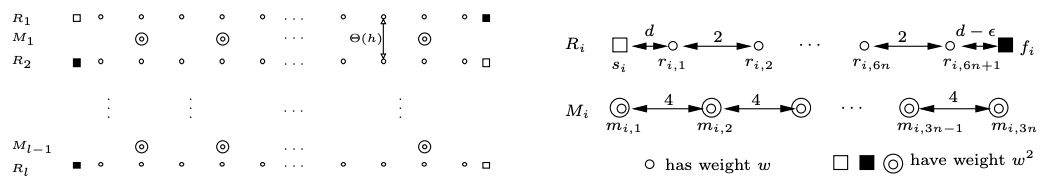
\includegraphics[width=15cm]{chapter_1/files/vattani_fig1.png}
\centering
    \caption{On the left side, the grid of points $H_{l,n}$. On the right, details of the rows \cite{vattani}}
    \label{fig:vattani1}
\end{figure}

\begin{definition}\label{def1}
Define two possible $(3n+2)$-clusterings of $R_i$ ($1\le i \le l$).

$A$: For $1\le j \le 3n$, the $j^{\text{th}}$ cluster of $R_i$ is $\{r_{i,2j-1},r_{i,2j}\}$. It also has the clusters $\{s_i\}$ and $\{r_{i,6n+1},f_i\}$.

$B$: For $1\le j \le 3n$, the $j^{\text{th}}$ cluster of $R_i$ is $\{r_{i,2j},r_{i,2j+1}\}$. It also has the clusters $\{s_i,r_{i,1}\}$ and $\{f_i\}$.
\end{definition}

\begin{definition}\label{def2}
We say that a $k$-clustering of $H_{l,n}$ is ``nice'' if each $m_{i,j}$ is a singleton cluster and each $R_i$ is grouped in an $A$-clustering or in a $B$-clustering.
\end{definition}

\begin{lemma}\label{lem1}
A nice $k$-clustering of $H_{l,n}$ with $t$ rows grouped in an $A$-clustering costs $L_1-t\alpha$.
\end{lemma}

A nice clustering, defined in Definition \ref{def2}, corresponds naturally to the $k$ that was chosen, since there are $l-1$ $M$ rows, each with $3n$ points in singleton clusters, and $l$ $R$ rows, with $3n+2$ clusters each, corresponding to $3n+1$ clusters with two consecutive points and 1 cluster with one point (whether $s_i$ or $f_i$ is the singleton cluster depends on whether $R_i$ is in an $A$ or $B$ clustering, respectively). Note an $A$ clustering saves exactly $\alpha$ cost compared to a $B$ clustering.

\begin{lemma}\label{lem2}
For $w=\text{poly}(n,l)$ large enough, any non-nice $k$-clustering of $H_{l,n}$ costs at least $L_1+\Omega(w)$. On the other hand, any nice $k$-clustering of $H_{l,n}$ costs at most $L_1$.
\end{lemma}

Lemma \ref{lem2} establishes that for $w$ large enough, any optimal clustering of $H_{l,n}$ must be ``nice.'' Note that Lemma \ref{lem1} allows us to make the stronger statement that in additional to the optimal clustering being nice, all $R_i$'s will be grouped in $A$ clusterings, for a total cost of $L_1-l\alpha$.

%However, note that soon we will be adding more points to create $G_{l,n}\cup X$, and for this augmented instance, we will argue that iff the corresponding X3C instance is satisfiable, the optimal clustering will have exactly $n$ $R_i$ in the $A$ clustering and the remaining $R_i$ in the $B$ clustering.

Now we construct the $k$-means instance corresponding to the reduction. It contains the points $G_{l,n}\cup X$, where $G_{l,n}$ is a slightly modified version of $H_{l,n}$ and the set $X=\bigcup_{i=1}^l X_i$ depends on the X3C collection $\mathcal{C}$.

\begin{figure}
    \centering
    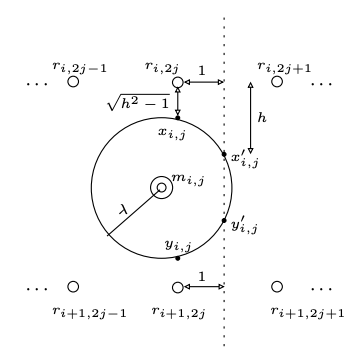
\includegraphics[width=6cm]{chapter_1/files/vattani_fig2.png}
\centering
    \caption{Close-up of $G_{l,n}\cup X$ \cite{vattani}}
    \label{fig:vattani2}
\end{figure}

Refer to Figure \ref{fig:vattani2} for details on $G_{l,n}$, where we set $\lambda=\Theta(h)$ (again, its exact value is only important to the proof of the lemmas which we omit here). The new grid $G_{l,n}$ is identical to $H_{l,n}$ except that the points in the rows in $M_i$ are no longer vertically aligned with the points in the rows $R_i$. The previous results about $H_{l,n}$ still apply to $G_{l,n}$, since the distance between rows is still $\Theta(h)$.

Now we define the set $X$. The spots $x_{i,j},x'_{i,j},y_{i,j},y'_{i,j}$ ($1\le i \le l-1$ and $1 \le j \le 3n$) are not all points in $X$ but rather possible positions of points, where exactly half of each group of four points will be occupied: $x_{i,j}\in X_i\iff j\not\in S_i$; $x'_{i,j}\in X_i\iff j\in S_i$; $y_{i,j}\in X_i\iff j\not\in S_{i+1}$; $y'_{i,j}\in X_i\iff j\in S_{i+1}$. All these points have weight $1$.

We set the number of clusters to be the same $k$ as before, and the cost limit to $L=L_1+L_2-n\alpha$ where $L_2=6n(l-1)h^2\frac{2w}{2w+1}$.

\begin{definition}\label{def3}
A cluster $C$ is ``good'' for a point $z\not\in C$ if adding $z$ to $C$ increases the cost by exactly $h^2\frac{2w}{2w+1}$.
\end{definition}

\begin{lemma}\label{lem3}
For any $1\le j \le 3n$, $1\le i \le l-1$, the following holds:
\begin{itemize}
    \item The clusters $\{m_{i,j}\}$, $\{r_{i,2j-1},r_{i,2j}\}$, and $\{r_{i,2j},r_{i,2j+1}\}$ are good for $x_{i,j}$.
    \item The clusters $\{m_{i,j}\}$, $\{r_{i+1,2j-1},r_{i+1,2j}\}$, and $\{r_{i+1,2j},r_{i+1,2j+1}\}$ are good for $y_{i,j}$.
    \item The clusters $\{m_{i,j}\}$ and $\{r_{i,2j},r_{i,2j+1}\}$ are good for $x'_{i,j}$.
    \item The clusters $\{m_{i,j}\}$ and $\{r_{i+1,2j},r_{i+1,2j+1}\}$ are good for $y'_{i,j}$.
\end{itemize}
\end{lemma}

Note that we have added $\abs{X}=6n(l-1)$ additional points and that if $j\in S_i$, then the corresponding $x'_{i,j}$ and $y'_{i-1,j}$ will only have a ``good'' cluster in $R_i$ if $R_i$ has a $B$ clustering, whereas $j\not\in S_i$ does not impose this restriction on the corresponding $x_{i,j}$ and $y_{i-1,j}$, i.e. $R_i$ can have either an $A$ or $B$ clustering.

Definition \ref{def3} and Lemma \ref{lem3} justify the choice of $L_2$. Also, from Figure \ref{fig:vattani2}, we can verify that the ``good'' clusters mentioned in Lemma \ref{lem3} are indeed the closest clusters to the spots $x_{i,j},x'_{i,j},y_{i,j},y'_{i,j}$.

\begin{lemma}\label{lem4}
Consider any optimal $k$-clustering of $G_{l,n}\cup X$. Then for $w=\text{poly}(n,l)$ large enough, the clustering induced on $G_{l,n}$ is nice and the points in $X$ are in different good clusters.
\end{lemma}

See \cite{vattani} for proofs of Lemmas \ref{lem1}, \ref{lem2}, \ref{lem3}, and \ref{lem4}. The following final lemma contains the reduction.

\begin{lemma}\label{lem5}
The set $G_{l,n}\cup X$ has a $k$-clustering of cost less or equal to $L$ if and only if there is an exact cover $\mathcal{F}\subseteq \mathcal{C}$ for the X3C instance.
\end{lemma}

\begin{proof}
$(\implies)$ Suppose we have an optimal $k$-clustering with cost $\le L$. Define $\mathcal{F}=\{S_i:R_i\text{ is grouped in an $A$ clustering}\}$. We argue that $\mathcal{F}$ is an exact cover of $U$. Note that $|\mathcal{F}|\ge n$ since $L = L_1+L_2-n\alpha$. It is sufficient to prove that the sets in $\mathcal{F}$ do not overlap, since this means that $|\mathcal{F}| = n$ and furthermore $\bigcup_{S\in\mathcal{F}}S=U$. 

Consider some $S_i\in\mathcal{F}$ and some $j\in S_i$. Since we know that $R_i$ has an $A$-clustering, the $j^{\text{th}}$ cluster of $R_i$ is not a good cluster for any point in $X$. Then we make a pigeonhole-like argument: each $j$ ($1\le j \le 3n$) corresponds to $2(l-1)$ points in $X$. For these points, there are $l-1$ ``good'' clusters in $M$ rows and $l$ ``good'' clusters in $R$ rows (corresponding to the $j^{\text{th}}$ cluster in $R_i$ for $1\le i\le l$). So if the $j^{\text{th}}$ cluster in $R_i$ is not occupied by any point, then the $j^{\text{th}}$ cluster in all $R_{i'}$, $i'\ne i$, must be occupied by some point. For a given $i'\ne i$, the only candidates are the points in $X$ with the subscript $_{i',j}$, and therefore it must be that either $R_{i'}$ has a $B$-clustering (allowing for both $x/y$ or $x'/y'$ type points) or $j\not\in S_{i'}$, and then we know that the points will be the less restrictive $x/y$ type. This proves that $j\not\in S_{i'}$ for any $S_{i'}\in\mathcal{F}$ where $i'\ne i$, i.e. the sets in $\mathcal{F}$ do not overlap.

$(\impliedby)$ Suppose X3C has an exact cover $\mathcal{F}$. We define a $k$-clustering for $G_{l,n}\cup X$. Place all points $m_{i,j}$ into different singleton clusters. For each $1\le i \le l$, make $R_i$ an $A$-clustering if $S_i\in\mathcal{F}$ and a $B$-clustering otherwise. For each $1\le j \le 3n$, let $i(j)$ be the (unique) index such that $j\in S_{i(j)}$ and $S_{i(j)}\in\mathcal{F}$. For each $i<i(j)$, merge $x_{i,j}$ (or $x'_{i,j}$) with the $j^{\text{th}}$ cluster of $R_i$ and merge $y_{i,j}$ (or $y'_{i,j}$) with $\{m_{i,j}\}$. For each $i\ge i(j)$, merge $x_{i,j}$ (or $x'_{i,j}$) with $\{m_{i,j}\}$ and merge $y_{i,j}$ (or $y'_{i,j}$) with the $j^{\text{th}}$ cluster of $R_{i+1}$.

We will show that this assignment has cost at most $L$, which means that the answer to our $k$-means decision problem is yes. This happens if we have a ``nice'' clustering on the points in $G_{l,n}$, there are $n$ $R_i$ rows in $A$ clusterings, and all points in $X$ are assigned to different good clusters. The first two are explicitly satisfied in the construction; we only need to verify that in cases where we assigned $x'_{i,j}$ (resp. $y'_{i,j}$) where $1\le i < i(j)$ (resp. $i\ge i(j)$), it was indeed to a good cluster. However, if $x'_{i,j}$ (resp. $y'_{i,j}$) $\in X_i$, then $j\in S_i$ (resp. $S_{i+1}$), and since the sets in $\mathcal{F}$ are nonoverlapping, this means $S_i$ (resp. $S_{i+1}$) $\not\in\mathcal{F}$, and therefore $R_i$ (resp. $R_{i+1}$) is a $B$ clustering. Therefore all points were assigned to good clusters.
\end{proof}
